\section{Weighted Struck}

\begin{frame}
    \frametitle{Weighted structured output tracking with kernels}
    \begin{itemize}
        \item Add a scalar weight.
            \begin{align}
                F\left(\mathbf{x}, \mathbf{y}\right) &= \sum_{i, \mathbf{\bar{y}}} \beta_i^\mathbf{\bar{y}}
                    \langle \kappa\left(\mathbf{x}_i, \mathbf{\bar{y}}\right),
                    \kappa\left(\mathbf{x}, \mathbf{y}\right) \rangle
                    \tag{\ref{eq:discriminant_function}} \\
                F\left(\mathbf{x}, \mathbf{y}\right) &= \alert{s(\mathbf{y})} \sum_{i, \mathbf{\bar{y}}} \beta_i^\mathbf{\bar{y}}
                    \langle \kappa\left(\mathbf{x}_i, \mathbf{\bar{y}}\right),
                    \kappa\left(\mathbf{x}, \mathbf{y}\right) \rangle
            \end{align}
    \end{itemize}
\end{frame}

\begin{frame}
    \frametitle{Fuzziness function}
    \begin{align}
        s(\mathbf{y}) &= 1 - \frac{\|\mathbf{y}\|}{\|\mathbf{y}_{max}\|} \\
        \mathbf{y}_{max} &= (width_I, height_I)
    \end{align}
\end{frame}

\begin{frame}
    \frametitle{Sampling locations}
    \begin{columns}
        \begin{column}{0.5\textwidth}
            Original Struck

            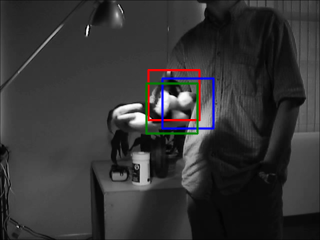
\includegraphics[width=\textwidth]{sylv}
        \end{column}
        \begin{column}{0.5\textwidth}
            Weighted Struck

            \includegraphics[width=\textwidth]{sylv_fuzzy}
        \end{column}
    \end{columns}
\end{frame}

